%%%%%%%%%%%%%%%%%%%%%%%%%%%%%%%%%%%%%%%%%%%%%%%%%%%%%%%%%%%%%%%%%%%%%%%%%%%%%%%%%%
\begin{frame}[fragile]\frametitle{}
\begin{center}
{\Large Distributions}
\end{center}
\end{frame}


%%%%%%%%%%%%%%%%%%%%%%%%%%%%%%%%%%%%%%%%%%%%%%%%%%%%%%%%%%%%%%%%%%%%%%%%
\begin{frame}[fragile]\frametitle{What is a Statistical Distribution?}

Example
\begin{columns}
    \begin{column}[T]{0.6\linewidth}
	\begin{itemize}
	\item Say, we are measuring height of people and we plotted histogram.
	\item Measurements in the middle are more than at the ends (extreme values).
	\item If we decrease the bin size to very small width, and with lots of observations, we will get a continuous curve approximating the tops.
	\item The curve gives a general sense, so we still can calculate frequencies of the missing observations.
	\end{itemize}

    \end{column}
    \begin{column}[T]{0.4\linewidth}
      \begin{center}
      \includegraphics[width=\linewidth,keepaspectratio]{statq10}
	  
	  \includegraphics[width=\linewidth,keepaspectratio]{statq11}
	  
	  \includegraphics[width=\linewidth,keepaspectratio]{statq12}	  
	  	\end{center}
    \end{column}

  \end{columns}
  
Thats `normal' distribution.

\tiny{(Ref: StatQuest: What is a statistical distribution? - Josh Starmer )}
\end{frame}


%%%%%%%%%%%%%%%%%%%%%%%%%%%%%%%%%%%%%%%%%%%%%%%%%%%%%%%%%%%%%%%%%%%%%%%%
\begin{frame}[fragile]\frametitle{`Normal' or `Gaussian' Distribution}
Also called `Bell Curve'.

\begin{columns}
    \begin{column}[T]{0.6\linewidth}
	\begin{itemize}
	\item More people are in the middle region. 
	\item Thats also a relative probability saying that its more likely to find someone of average height.
	\item Its less likely (low probability) to find someone very tall or very short.
	\item Another example: two normal distributions of the height of male humans when born and as adults.
	\item For babies, almost all of them have similar heights (20 inches), but as adults variations are more.
	\end{itemize}

    \end{column}
    \begin{column}[T]{0.4\linewidth}
      \begin{center}
      \includegraphics[width=\linewidth,keepaspectratio]{statq13}
	  
	  \includegraphics[width=\linewidth,keepaspectratio]{statq14}
	   
	  	\end{center}
    \end{column}

  \end{columns}
  
\tiny{(Ref: StatQuest: What is a statistical distribution? - Josh Starmer )}
\end{frame}


%%%%%%%%%%%%%%%%%%%%%%%%%%%%%%%%%%%%%%%%%%%%%%%%%%%%%%%%%%%%%%%%%%%%%%%%
\begin{frame}[fragile]\frametitle{`Normal' or `Gaussian' Distribution}
      \begin{center}
      \includegraphics[width=0.8\linewidth,keepaspectratio]{statq15}
	  
	  \includegraphics[width=0.8\linewidth,keepaspectratio]{statq16}
    \end{center}
		

\tiny{(Ref: StatQuest: What is a statistical distribution? - Josh Starmer )}
\end{frame}

%%%%%%%%%%%%%%%%%%%%%%%%%%%%%%%%%%%%%%%%%%%%%%%%%%%%%%%%%%%%%%%%%%%%%%%%
\begin{frame}[fragile]\frametitle{Width of the curve is represented by Standard deviation.}

      \begin{center}
  
	   
	  \includegraphics[width=0.8\linewidth,keepaspectratio]{statq17}
	   
      \includegraphics[width=0.8\linewidth,keepaspectratio]{statq18}	   
	  	\end{center}
		

\tiny{(Ref: StatQuest: What is a statistical distribution? - Josh Starmer )}
\end{frame}

%%%%%%%%%%%%%%%%%%%%%%%%%%%%%%%%%%%%%%%%%%%%%%%%%%%%%%%%%%%%%%%%%%%%%%%%
\begin{frame}[fragile]\frametitle{`Normal' or `Gaussian' Distribution}
      \begin{center}

	  
	  \includegraphics[width=0.8\linewidth,keepaspectratio]{statq19}
	   
   
	  \includegraphics[width=0.8\linewidth,keepaspectratio]{statq20}
	   
	  	\end{center}
		

\tiny{(Ref: StatQuest: What is a statistical distribution? - Josh Starmer )}
\end{frame}

%%%%%%%%%%%%%%%%%%%%%%%%%%%%%%%%%%%%%%%%%%%%%%%%%%%%%%%%%%%%%%%%%%%%%%%%
\begin{frame}[fragile]\frametitle{`Normal' or `Gaussian' Distribution}

	\begin{itemize}
	\item Normal Distribution is observed widely in nature, eg heights, weights, incomes, etc
	\item The reason behind this is: The Central Limit Theorem.
	\item Briefly, if you plot averages of samples, they form normal distribution.
	
	\end{itemize}

  
\tiny{(Ref: StatQuest: What is a statistical distribution? - Josh Starmer )}
\end{frame}

%%%%%%%%%%%%%%%%%%%%%%%%%%%%%%%%%%%%%%%%%%%%%%%%%%%%%%%%%%%
\begin{frame}
\frametitle{Mathematically, The normal distribution}

The normal (or Gaussian) distribution is a continuous, symmetric distribution.

The {\bf standard normal distribution}, denoted $N(0,1)$ is a normal
distribution with mean 0 and variance 1.  The normal distribution
$N(\mu, \sigma^2)$ has mean $\mu$ and variance $\sigma^2$.

From the properties of expected values and standard deviations given earlier:

\begin{itemize}

\item If $Z$ is standard normal, then $\mu + \sigma Z$ is
  $N(\mu,\sigma^2$).

\item If $Z$ is $N(\mu, \sigma^2)$, then $(Z-\mu)/\sigma$ is standard
  normal.

\end{itemize}

\end{frame}

%%%%%%%%%%%%%%%%%%%%%%%%%%%%%%%%%%%%%%%%%%%%%%%%%%%%%%%%%%%%%%%%%%%%%%%%
\begin{frame}[fragile]\frametitle{Sampling a Distribution}
\begin{columns}
    \begin{column}[T]{0.6\linewidth}
	\begin{itemize}
	\item If we take one sample from a Normal Distribution, most likely it will be a value near middle.
	\item Once in a while we may get values from ends as well.
	\item Why do you take samples: to explore the statistics.
	\item Rather than measuring all, to explore using only a few values.
	\end{itemize}

    \end{column}
    \begin{column}[T]{0.4\linewidth}
      \begin{center}
      \includegraphics[width=\linewidth,keepaspectratio]{statq21}
	  
	  \includegraphics[width=\linewidth,keepaspectratio]{statq22}
	   
	  	\end{center}
    \end{column}

  \end{columns}
  
\tiny{(Ref: StatQuest: What is a statistical distribution? - Josh Starmer )}
\end{frame}

%%%%%%%%%%%%%%%%%%%%%%%%%%%%%%%%%%%%%%%%%%%%%%%%%%%%%%%%%%%%%%%%%%%%%%%%
\begin{frame}[fragile]\frametitle{Sampling a Distribution}
\begin{columns}
    \begin{column}[T]{0.6\linewidth}
	\begin{itemize}
	\item Tests can be used to see if the samples represent the original population data.
	\item We can measure similarity between two samples as well, by t-test.
	\item Since the original distribution form both is same, should give large p value (meaning both are mostly same)
	\item With just 3 samples for different distributions if p value is small, then increase the sample size.
	\end{itemize}

    \end{column}
    \begin{column}[T]{0.4\linewidth}
      \begin{center}
      \includegraphics[width=\linewidth,keepaspectratio]{statq23}
	  
	  \includegraphics[width=\linewidth,keepaspectratio]{statq24}
	   
	  	\end{center}
    \end{column}

  \end{columns}
  
 Calculating normal probabilities meaning sampling normal distribution.
 
\tiny{(Ref: StatQuest: What is a statistical distribution? - Josh Starmer )}
\end{frame}



%%%%%%%%%%%%%%%%%%%%%%%%%%%%%%%%%%%%%%%%%%%%%%%%%%%%%%%%%%%
\begin{frame}[fragile]
\frametitle{Calculating normal probabilities}

Suppose we have a random variable $T$ which has mean $\mu$ and
variance $\sigma^2$.  If we are willing to assume $T$ is normal, how
can we calculate $P(T>c)$ for some constant $c$?

Normal probability tables are available on the web and in most
statistics software packages.  Often only a table for the standard
normal distribution is available, but this is sufficient, since

\vspace{-0.5cm}

\begin{eqnarray*}
P(T>c) &=& P((T-\mu)/\sigma > (c-\mu)/\sigma)\\ &=& 1 - P(Z \le
(c-\mu)/\sigma).
\end{eqnarray*}

Thus we can look up the value of $(c-\mu)/\sigma$ in a standard normal
probability, table or use a software package, e.g. in R we would use

\begin{lstlisting}
1 - pnorm((c-mu)/s)
\end{lstlisting}

\end{frame}

%%%%%%%%%%%%%%%%%%%%%%%%%%%%%%%%%%%%%%%%%%%%%%%%%%%%%%%%%%%
\begin{frame}
\frametitle{Normal distribution rules of thumb}

\begin{itemize}

\item The normal distribution is symmetric -- around half of a normal
sample lies below the mean and half lies above the mean.

\item Around 68\% of a normal sample lies within one standard
deviation of the mean.  For example, if we have 1000 points from a
normal distribution with mean $10$ and variance $4$, around 680 of the
points will lie between 8 and 12.

\item Around 95\% of a normal sample lies within two standard
  deviations of the mean.  Continuing with the previous example,
  around 950 of the points will lie between 6 and 14.

\item Around 99\% of a normal sample lies within three standard
  deviations of the mean.  Continuing with the previous example,
  around 990 of the points will lie between 4 and 16.

\end{itemize}

\end{frame}



%%%%%%%%%%%%%%%%%%%%%%%%%%%%%%%%%%%%%%%%%%%%%%%%%%%%%%%%%%%%%%%%%%%%%%%%
\begin{frame}[fragile]\frametitle{Normal Distribution}
The classic bell curve-shaped distribution and is completely determined by two parameters: its mean (mu) and its standard deviation	 (sigma).
\begin{center}
\includegraphics[width=0.6\linewidth,keepaspectratio]{normdisteq}
\end{center}
Implement. 

Use \lstinline|math.sqrt| and \lstinline|math.pi| as well as \lstinline|matplotlib.pyplot| for plotting
\begin{lstlisting}
def normal_pdf(x, mu=0, sigma=1):
	:
	return v
\end{lstlisting}
\end{frame}

%%%%%%%%%%%%%%%%%%%%%%%%%%%%%%%%%%%%%%%%%%%%%%%%%%%%%%%%%%%%%%%%%%%%%%%%
\begin{frame}[fragile]\frametitle{Normal Distribution}
Data and plotting routine
\begin{lstlisting}
xs=[x	/10.0 for x in range(-50, 50)]

plt.plot(xs,[normal_pdf(x,sigma=1) for x in xs],'-')
plt.plot(xs,[normal_pdf(x,sigma=2) for x in xs],'--')
plt.plot(xs,[normal_pdf(x,sigma=0.5) for x in xs],':')
plt.plot(xs,[normal_pdf(x,mu=-1) for x in xs],'-')
plt.legend()
plt.title("Normal pdfs")
plt.show()
\end{lstlisting}
\end{frame}

%%%%%%%%%%%%%%%%%%%%%%%%%%%%%%%%%%%%%%%%%%%%%%%%%%%%%%%%%%%%%%%%%%%%%%%%
\begin{frame}[fragile]\frametitle{Normal Distribution}
\begin{lstlisting}
import math
import matplotlib.pyplot as plt
def normal_pdf(x, mu=0, sigma=1):
	sqrt_two_pi = math.sqrt(2*math.pi)
	return	(math.exp(-(x-mu)**2/2/sigma**2) / (sqrt_two_pi* sigma))
\end{lstlisting}
\end{frame}

%%%%%%%%%%%%%%%%%%%%%%%%%%%%%%%%%%%%%%%%%%%%%%%%%%%%%%%%%%%%%%%%%%%%%%%%
\begin{frame}[fragile]\frametitle{Normal Distribution}
\begin{center}
\includegraphics[width=0.8\linewidth,keepaspectratio]{normdistplot}
\end{center}
\end{frame}


%%%%%%%%%%%%%%%%%%%%%%%%%%%%%%%%%%%%%%%%%%%%%%%%%%%%%%%%%%%
\begin{frame}
\frametitle{Log transforms}

Some quantities that vary over several orders of magnitude are best
analyzed on the log scale.

For example, if we observe these values:

$$
14,28,3,60,39,13,1,9,3,55
$$

We can take $\log_2$ to get their approximate values as powers of 2:

$$
3.8, 4.8, 1.6, 5.9, 5.3, 3.7, 0, 3.2, 1.6, 5.8.
$$

It usually doesn't matter what base is used, since we can convert from
one base to another by scaling:

$$
\log_b(x) = \log_a(x) / \log_a(b)
$$

\end{frame}

%%%%%%%%%%%%%%%%%%%%%%%%%%%%%%%%%%%%%%%%%%%%%%%%%%%%%%%%%%%
\begin{frame}
\frametitle{Symmetrizing effect of log transforms}

The log transform symmetrizes right-skewed distributions:

\begin{center}
\begin{tabular}{cc}
\scalebox{0.3}{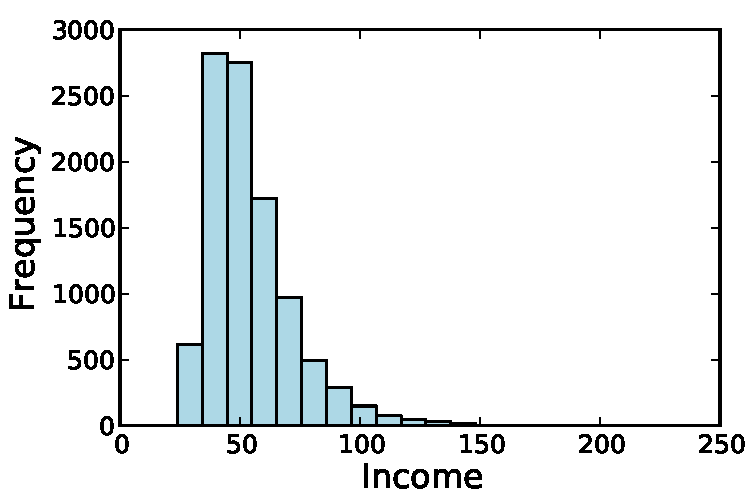
\includegraphics{042-1.pdf}} &
\scalebox{0.3}{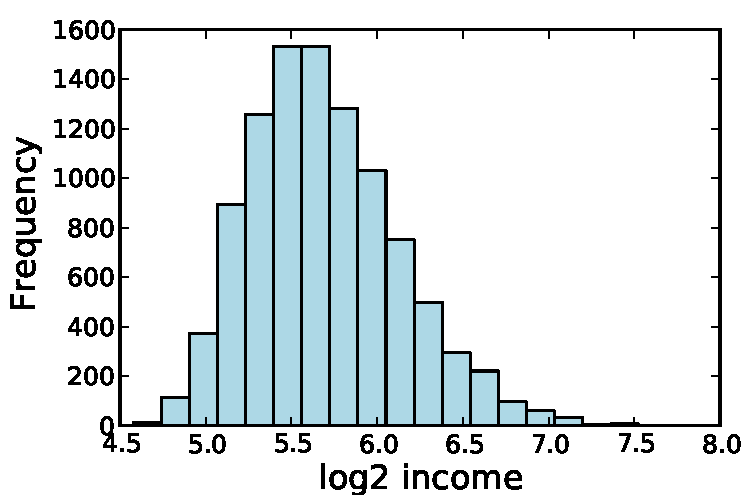
\includegraphics{042-2.pdf}} 
\end{tabular}
\end{center}

It's common to transform data to make it more symmetric, and usually
that's the right thing to do (but don't overdo it...).


\end{frame}

%%%%%%%%%%%%%%%%%%%%%%%%%%%%%%%%%%%%%%%%%%%%%%%%%%%%%%%%%%%
\begin{frame}
\frametitle{Properties of log transforms}

Remember the key properties of logarithms: 

$$\log(ab) = \log(a) + \log(b) \hspace{2cm} \log(a^b) = b\log(a).$$

As a consequence, if we take data $X_1, \ldots, X_n$ and scale it to
get $Z_i = cX_i$, then

$$
\log(Z_1), \ldots, \log(Z_n) = \log(c)+\log(X_1), \ldots, \log(c)+\log(X_n)
$$

Thus changing the units of the original data becomes a shift by
$\log(c)$ units for the log-transformed data.

\end{frame}

%%%%%%%%%%%%%%%%%%%%%%%%%%%%%%%%%%%%%%%%%%%%%%%%%%%%%%%%%%%
\begin{frame}
\frametitle{Mean values and log transforms}

If we observe data $X_1, \ldots, X_n$ and take a log transform to get
$Y_i = \log X_i$, then the mean value of the logged data is:

\begin{eqnarray*}
\bar{Y} &=& n^{-1}\sum_i Y_i\\
       &=& n^{-1}\sum_i \log X_i\\
       &=& n^{-1}\log(X_1 \cdot X_2 \cdots X_n)\\
       &=& \log\left((X_1 \cdot X_2 \cdots X_n)^{1/n}\right).
\end{eqnarray*}

$(X_1 \cdot X_2 \cdots X_n)^{1/n}$ is called the {\bf geometric mean}
of the $X_i$, so we see that the usual (arithmetic) mean of the log
transformed data is the log of the geometric mean of the untransformed
data.

\end{frame}


\begin{frame}
\frametitle{Log transforms}

We generally take the log of positive data that is substantially right
skewed.  If the data are roughly symmetrically distributed, there is
no need to take a log transform, and you cannot take a log transform
if any of the data values are less than or equal to zero.

\textcolor{blue}{\bf Examples:} We generally would log-transform
income but not age.


\end{frame}



%%%%%%%%%%%%%%%%%%%%%%%%%%%%%%%%%%%%%%%%%%%%%%%%%%%%%%%%%%%
\begin{frame}
\frametitle{Standardizing the sample mean}

Suppose we have an id sample of $n$ observations from a population
with mean $\mu$ and variance $\sigma^2$.

We know that $\bar{X}$ has mean $\mu$ and variance $\sigma^2/n$ (so
the standard deviation is $\sigma/\sqrt{n}$).  

The standardized sample mean is

$$
\frac{\bar{X}-\mu}{\sigma/\sqrt{n}} = \sqrt{n}\frac{\bar{X}-\mu}{\sigma}.
$$

\end{frame}


\begin{frame}
\frametitle{Example calculation with the normal distribution}

Suppose we have a sample $X_1, \ldots, X_{20}$ from a normal
population with mean zero.  We are told that the probability that
$|\bar{X}|$ is greater than 1 is 0.2.  What is the standard deviation
of the $X_i$?

Using the fact that the normal distribution is symmetric,

\begin{eqnarray*}
0.2 &=& P(|\bar{X}| > 1)\\ &=& P(\bar{X}>1) + P(\bar{X}<-1)\\ &=&
2P(\bar{X}>1)\\ &=&
2P(\sqrt{20}\bar{X}/\sigma>\sqrt{20}/\sigma)\\ &=& 2P(Z >
\sqrt{20}/\sigma).
\end{eqnarray*}

So $P(Z > \sqrt{20}/\sigma) = 0.1$.  Now if we look at a table of the
normal distribution, we see that the probability of a standard normal
value being bigger than 1.28 is 0.1, so $\sqrt{20}/\sigma = 1.28$, and
$\sigma = \sqrt{20}/1.28 \approx 3.49$.

\end{frame}


\begin{frame}
\frametitle{Exercises}

\begin{enumerate}

\item Suppose we observe a sample of 100 values from a normal
 population with mean 100 and standard deviation 10.  Around how many
 of the values will be greater than 110?

\item Suppose we observe a sample of 150 values from a normal
 population with mean 80 and standard deviation 12.  Write an R
 expression that will give the approximate number of values between
 75 and 85.

\item Suppose we observe a sample of 200 values from a normal
 distribution with mean zero.  Around 20 of the values that we
 observe are greater than 50.  Approximately what is the standard
 deviation of the population we are sampling from?

\end{enumerate}

\end{frame}


%%%%%%%%%%%%%%%%%%%%%%%%%%%%%%%%%%%%%%%%%%%%%%%%%%%%%%%%%%%%%%%%%%%%%%%%%%%%%%%%%%
\begin{frame}[fragile]\frametitle{}
\begin{center}
{\Large Normal Distribution in Practice}
\end{center}
\end{frame}


%%%%%%%%%%%%%%%%%%%%%%%%%%%%%%%%%%%%%%%%%%%%%%%%%%%%%%%%%%%
\begin{frame}
\frametitle{Normal Distribution in Practice}

\begin{itemize}
\item Applied to single variable continuous data e.g. heights of plants, weights of lambs, lengths of time
\item Used to calculate the probability of occurrences less than, more than, between given values e.g. 
\begin{itemize}
\item The probability that the plants will be less than 70mm
\item The probability that the lambs will be heavier than 70kg
\item The probability that the time taken will be between 10 and 12 minutes
\end{itemize}
\item Standard Normal tables give probabilities
\end{itemize}


{\tiny (Ref: Normal, Binomial, Poisson Distributions -  Lincoln University)}
\end{frame}

%%%%%%%%%%%%%%%%%%%%%%%%%%%%%%%%%%%%%%%%%%%%%%%%%%%%%%%%%%%
\begin{frame}
\frametitle{How to use Normal Distribution table?}

\begin{itemize}
\item First need to calculate how many standard deviations above (or below) the mean a
particular value is, i.e., calculate the value of the ``standard score'' or ``Z-score''.
\item Use the following formula to convert a raw data value, $X$, to a standard score:
$Z = \frac{(X - \mu)}{\sigma}$
\item eg. Suppose a particular population has $\mu= 4$ and $\sigma = 2$. Find the probability of a
randomly selected value being greater than 6
\item The Z score corresponding to $X = 6$ is $Z = \frac{(6 - 4)}{2} = 1$
\item $Z=1$ means that the value $X = 6$ is 1 standard deviation away from the mean
\item Use  standard normal tables to find $P(Z>1) = 0.6587$
\end{itemize}


{\tiny (Ref: Normal, Binomial, Poisson Distributions -  Lincoln University)}
\end{frame}

%%%%%%%%%%%%%%%%%%%%%%%%%%%%%%%%%%%%%%%%%%%%%%%%%%%%%%%%%%%
\begin{frame}
\frametitle{Example}
Wool fibre breaking strengths are normally distributed with mean $\mu = 23.56$ Newtons
and standard deviation, $\sigma = 4.55$.
What proportion of fibres would have a breaking strength of 14.45 or less? 
\begin{itemize}
\item Draw a diagram, label and shade area required

\begin{center}
\includegraphics[width=0.3\linewidth,keepaspectratio]{stats1}
\end{center}

\item Convert raw score $X$ to standard score $Z$: $Z = \frac{(14.45 - 23.56)}{4.55} = - 2.0$
\item That is, the raw score of 14.45 is equivalent to a standard score of -2.0.
\item It is negative because it is on the left hand side of the curve.
\item Use tables to find probability and adjust this result to required probability: 
\begin{align*}
p(X < 14.45) = p(Z ,-2.0) &= 0.5 - p(0< Z < 2)\\
&= 0.5 - 0.4772\\
&=0.0228
\end{align*}
\end{itemize}


{\tiny (Ref: Normal, Binomial, Poisson Distributions -  Lincoln University)}
\end{frame}


%%%%%%%%%%%%%%%%%%%%%%%%%%%%%%%%%%%%%%%%%%%%%%%%%%%%%%%%%%%
\begin{frame}
\frametitle{Inverse Process}
To find a value for X, corresponding to a given probability
\begin{itemize}
\item Draw a diagram and label
\item Shade area given as per question
\item Use probability tables to find Z -score
\item Convert standard score $Z$ to raw score $X$ using inverse formula
\end{itemize}


{\tiny (Ref: Normal, Binomial, Poisson Distributions -  Lincoln University)}
\end{frame}

%%%%%%%%%%%%%%%%%%%%%%%%%%%%%%%%%%%%%%%%%%%%%%%%%%%%%%%%%%%
\begin{frame}
\frametitle{Example}
Carrots entering a processing factory have an average length of 15.3 cm, and
standard deviation of 5.4 cm. If the lengths are approximately normally distributed,
what is the maximum length of the lowest 5\% of the load?
(i.e., what value cuts off the lowest 5 \%?)
\begin{itemize}
\item Draw a diagram, label and shade area required

\begin{center}
\includegraphics[width=0.3\linewidth,keepaspectratio]{stats2}
\end{center}

\item Use standard Normal tables to find the Z -score corresponding to this area of probability. 
\item Convert the standard score $Z$ to a raw score $X$ using the inverse formula: $X = Z \times \sigma + \mu$
\item For $p(Z < z) = 0.05$ the Normal tables give the corresponding z-score as -1.645.
(Negative because it is left of the mean.)
\item Hence the raw score is 
\begin{align*}
X &= Z \times \sigma + \mu\\
&= -1.645 \times 5.44 + 15.3\\
&=6.4
\end{align*}
\item ie the lowest maximum length is 6.4cm
\end{itemize}


{\tiny (Ref: Normal, Binomial, Poisson Distributions -  Lincoln University)}
\end{frame}

%%%%%%%%%%%%%%%%%%%%%%%%%%%%%%%%%%%%%%%%%%%%%%%%%%%%%%%%%%%%%%%%%%%%%%%%%%%%%%%%%%
\begin{frame}[fragile]\frametitle{}
\begin{center}
{\Large Binomial Distribution}
\end{center}
\end{frame}

%%%%%%%%%%%%%%%%%%%%%%%%%%%%%%%%%%%%%%%%%%%%%%%%%%%%%%%%%%%%%%%%%%%%%%%%
\begin{frame}[fragile]\frametitle{Binomial Distribution}
Example: Which drink people prefer: Tea or Coffee?


	\begin{itemize}
	\item If 4 out of 7 people prefer Tea, do we say that general population prefers Tea?
	\item Or it could be that people in general do not have any preference over each other and this observation is just due to random chance and a small sample size.
	\item If we had surveyed another set of 7 people, we have have had 4 people preferring Coffee.
	\item In such Yes/No outcomes, we use Binomial distribution as the model.
	\item We will see how data fits the model.
	\item If the model is a poor fit, we will reject the idea that both tea and coffee are loved equally (ie there is no preference within them).
	\end{itemize}



  
\tiny{(Ref: StatQuest: The Binomial Distribution and Test, Clearly Explained!!! - Josh Starmer )}
\end{frame}

%%%%%%%%%%%%%%%%%%%%%%%%%%%%%%%%%%%%%%%%%%%%%%%%%%%%%%%%%%%%%%%%%%%%%%%%
\begin{frame}[fragile]\frametitle{Binomial Distribution}
Example: Which drink people prefer: Tea or Coffee?


	\begin{itemize}
	\item If people really did not prefer Tea over Coffee (and vice versa), then we will assume that there is 50\% chance they will pick Tea and 50\% chance that they will pick Coffee.
	\item Out of 3 people, lets calculate probability of first 2 people choosing Tea and the last one choosing Coffee.
	\item 1st Tea: 0.5
	\item 2nd Tea: 0.5
	\item 3rd Coffee: 0.5
	\item Total: $0.5 \times 0.5 \times 0.5 = 0.125$ 
	\item This is true for 3 cases: TTC, TCT, CTT
	\item So, Probability that any 2 out of 3 people preferring Ta is sum of these = 0.125 + 0.125 + 0.125 = 0.375
	\item This is readily given by $p(x|n,p) = (\frac{n!}{x!(n-x)!})p^x(1-p)^{n-x}$
	\end{itemize}

 
\tiny{(Ref: StatQuest: The Binomial Distribution and Test, Clearly Explained!!! - Josh Starmer )}
\end{frame}

%%%%%%%%%%%%%%%%%%%%%%%%%%%%%%%%%%%%%%%%%%%%%%%%%%%%%%%%%%%%%%%%%%%%%%%%
\begin{frame}[fragile]\frametitle{Binomial Distribution}
$p(x|n,p) = (\frac{n!}{x!(n-x)!})p^x(1-p)^{n-x}$


	\begin{itemize}
	\item x: number of people preferring Tea (2)
	\item n : total number of people we asked (3)
	\item p: probability that someone will pick Tea (0.5)
	\item The first part of the formula is just combinations formula, how many ways 2 things can be arranged out of 3. Its $= (\frac{3!}{2!(3-2)!})=3$.
	\item $p^x$ shows Tea probability x times, ie $p^x = 0.5^2 = 0.25$
	\item $(1-p)^{n-x}$ shows the remaining, ie coffee's probability $(1-0.5)^{3-2} = 0.5$
	\item So, the probability of x( the number of people who prefer Tea), given n (the total number of people asked) and p (probability of picking Tea) is $= (\frac{3!}{2!(3-2)!})(0.5)^x(1-0.5)^{3-2}$
	\end{itemize}

 
\tiny{(Ref: StatQuest: The Binomial Distribution and Test, Clearly Explained!!! - Josh Starmer )}
\end{frame}

%%%%%%%%%%%%%%%%%%%%%%%%%%%%%%%%%%%%%%%%%%%%%%%%%%%%%%%%%%%%%%%%%%%%%%%%
\begin{frame}[fragile]\frametitle{Binomial Distribution}
Going back to the original example: out of 7 , 4 prefer Tea. Can we say population prefers Tea?


	\begin{itemize}
	\item x: 4
	\item n : 7
	\item p: 0.5
	\item So, the probability someone randomly would pick Tea is $= (\frac{7!}{4!(7-4)!})(0.5)^4(1-0.5)^{7-4} = 35 \times 0.5^4(1-0.5)^3 = 0.273$
	\item Whats the p value of 4 of 7 people preferring Tea? It is the probability of 4 of 7 people preferring Tea over Coffee, plus the probabilities of all other possibilities that are equally likely or rarer.
	\item Means, we need to calculate, TTTTCCC,TTTTTCC,TTTTTTC,TTTTTTT. First is observed, reaming three are rare possibilities.
	\item We will also need probabilities CCCCTTT, CCCCCTT, CCCCCCT, CCCCCCC. With this we are calculating two sided (tailed) p value.
	\item Tea heavy arrangements give $= 0.273 + 0.164 + 0.055 + 0.008$ similarly for Coffee heavy arrangements. Total probability $0.5 + 0.5 = 1$
	\item Thus this is a good fit, meaning both Tea and Coffee are equally preferred.
	\item 
	\end{itemize}

 
\tiny{(Ref: StatQuest: The Binomial Distribution and Test, Clearly Explained!!! - Josh Starmer )}
\end{frame}


%%%%%%%%%%%%%%%%%%%%%%%%%%%%%%%%%%%%%%%%%%%%%%%%%%%%%%%%%%%
\begin{frame}
\frametitle{Binomial Distribution in Practice}

\begin{itemize}
\item Applied to single variable discrete data where results are the numbers of
``successful outcomes'' in a given scenario. 
\begin{itemize}
\item Number of times the lights are red in 20 sets of traffic lights
\item Number of students with green eyes in a class of 40
\item Number of plants with diseased leaves from a sample of 50 plants
\end{itemize}
\item Used to calculate the probability of occurrences exactly, less than, more than,
between given values
\begin{itemize}
\item The probability that the number of red lights will be exactly 5
\item The probability that the number of green eyed students will be less than 7
\item The probability that the number of diseased plants will be more than 10
\end{itemize}
\end{itemize}


{\tiny (Ref: Normal, Binomial, Poisson Distributions -  Lincoln University)}
\end{frame}


%%%%%%%%%%%%%%%%%%%%%%%%%%%%%%%%%%%%%%%%%%%%%%%%%%%%%%%%%%%
\begin{frame}
\frametitle{Binomial Distribution in Practice}

\begin{center}
\includegraphics[width=0.8\linewidth,keepaspectratio]{stats3}
\end{center}

Read as “the probability of getting $x$ successes is equal to the number of ways of choosing ``$x$  successes from n trials'' times ``the probability of success to
the power of the number of successes required'' times ''the probability of failure to
the power of the number of resulting failures.''


{\tiny (Ref: Normal, Binomial, Poisson Distributions -  Lincoln University)}
\end{frame}


%%%%%%%%%%%%%%%%%%%%%%%%%%%%%%%%%%%%%%%%%%%%%%%%%%%%%%%%%%%
\begin{frame}
\frametitle{Example }

An automatic camera records the number of cars running a red light at an
intersection (that is, the cars were going through when the red light was against the
car). Analysis of the data shows that on average 15\% of light changes record a car
running a red light. Assume that the data has a binomial distribution. What is the
probability that in 20 light changes there will be exactly three (3) cars running a red
light?

\begin{itemize}
\item Write out the key statistics from the information given $p =0.15, n = 20, X = 3$
\item Apply the formula, substituting these values: $P(X=3) = {20 \choose 3} 0.15^3 0.85^{17} = 0.243$
\item That is, the probability that in 20 light changes there will be three (3) cars running a
red light is 0.24 (24\%)
\end{itemize}

{\tiny (Ref: Normal, Binomial, Poisson Distributions -  Lincoln University)}
\end{frame}


%%%%%%%%%%%%%%%%%%%%%%%%%%%%%%%%%%%%%%%%%%%%%%%%%%%%%%%%%%%%%%%%%%%%%%%%%%%%%%%%%%
\begin{frame}[fragile]\frametitle{}
\begin{center}
{\Large Poisson Distribution}
\end{center}
\end{frame}

%%%%%%%%%%%%%%%%%%%%%%%%%%%%%%%%%%%%%%%%%%%%%%%%%%%%%%%%%%%
\begin{frame}
\frametitle{Poisson Distribution in Practice}

This is often known as the distribution of rare events. Firstly, a Poisson process is
where DISCRETE events occur in a CONTINUOUS, but finite interval of time or
space. The following conditions must apply:


\begin{itemize}
\item For a small interval the probability of the event occurring is proportional to the size of the interval.
\item The probability of more than one occurrence in the small interval is negligible (i.e. they are rare events). Events must not occur simultaneously
\item Each occurrence must be independent of others and must be at random.
\item  The events are often defects, accidents or unusual natural happenings, such as
earthquakes, where in theory there is no upper limit on the number of events.
The interval is on some continuous measurement such as time, length or area
\end{itemize}


{\tiny (Ref: Normal, Binomial, Poisson Distributions -  Lincoln University)}
\end{frame}



%%%%%%%%%%%%%%%%%%%%%%%%%%%%%%%%%%%%%%%%%%%%%%%%%%%%%%%%%%%
\begin{frame}
\frametitle{Poisson Distribution in Practice}
\begin{itemize}
\item The parameter for the Poisson distribution is $\lambda$(lambda). 
\item It is the average or mean
number of occurrences over a given interval.
\item The probability function is $p(x) = \frac{e^{-\lambda}\lambda^x}{x!}$ for $x=0,1,2,\ldots$
\item Example: The average number of accidents at a level-crossing every year
is 5. Calculate the probability that there are exactly 3 accidents
there this year.
\item Here, $\lambda = 5$, and $x = 3$.
\item $p(X=3) = \frac{e^{-5}5^3}{3!} = 0.1404$
\item That is, there is a 14\% chance that there will be exactly 3 accidents there this year
\end{itemize}


{\tiny (Ref: Normal, Binomial, Poisson Distributions -  Lincoln University)}
\end{frame}